\documentclass[12pt]{article}
\usepackage{setspace}
\setlength{\parindent}{4em}
\usepackage{fancyvrb}
\usepackage{graphicx}
\usepackage{geometry}
\renewcommand\thesection{\arabic{section}}
\renewcommand\thesubsection{\thesection.\arabic{subsection}}
\geometry{letterpaper, portrait, margin=1in}

%%%Title Page%%%
\title{\vspace{3cm}Lab 04\bigbreak Designing the Controller of the CPU}
\author{
{\normalsize
\begin{tabular}{l r r}
 & \textbf{Ryan Cruz} & \textbf{Zachary Davis}\\
\textbf{Category} & ryan.cruz25@uga.edu & zachdav@uga.edu\\
\hline
Pre-lab 						  & 50 & 50\\
In-lab Module \& Testbench Design & 50 & 50\\
In-lab Testbench Sim. \& Analysis & 50 & 50\\
In-lab FPGA Synthesis \& Analysis & 50 & 50\\
Lab Report Writing 				  & 50 & 50\\
\end{tabular}
}}
%%%%%%%%%%%%%%%%%

\begin{document}
\maketitle
\newpage
\setstretch{2.5} % for custom spacing
\tableofcontents
\setstretch{1} % for custom spacing
\newpage

\section{Lab Purpose} \vspace{-.7cm} \line(1,0){470}
	\paragraph{} In this lab we design the controller for the CPU, covering all possible states and transitions layed out by the control signal table we completed for prelab (Figure 2.). Like always, all test cases will be tested with a test bench and corresponding waveforms, shown in the Expiremental Results section.			
		
\section{Implementation Details} \vspace{-.7cm} \line(1,0){470}
		\subsection{Part 1}
        	\paragraph{Prelab} There were 3 parts to the prelab: Designing the FSM for the controller, the full control signal table, and the corresponding boolean equations for those signals.

		\begin{figure}[h]
			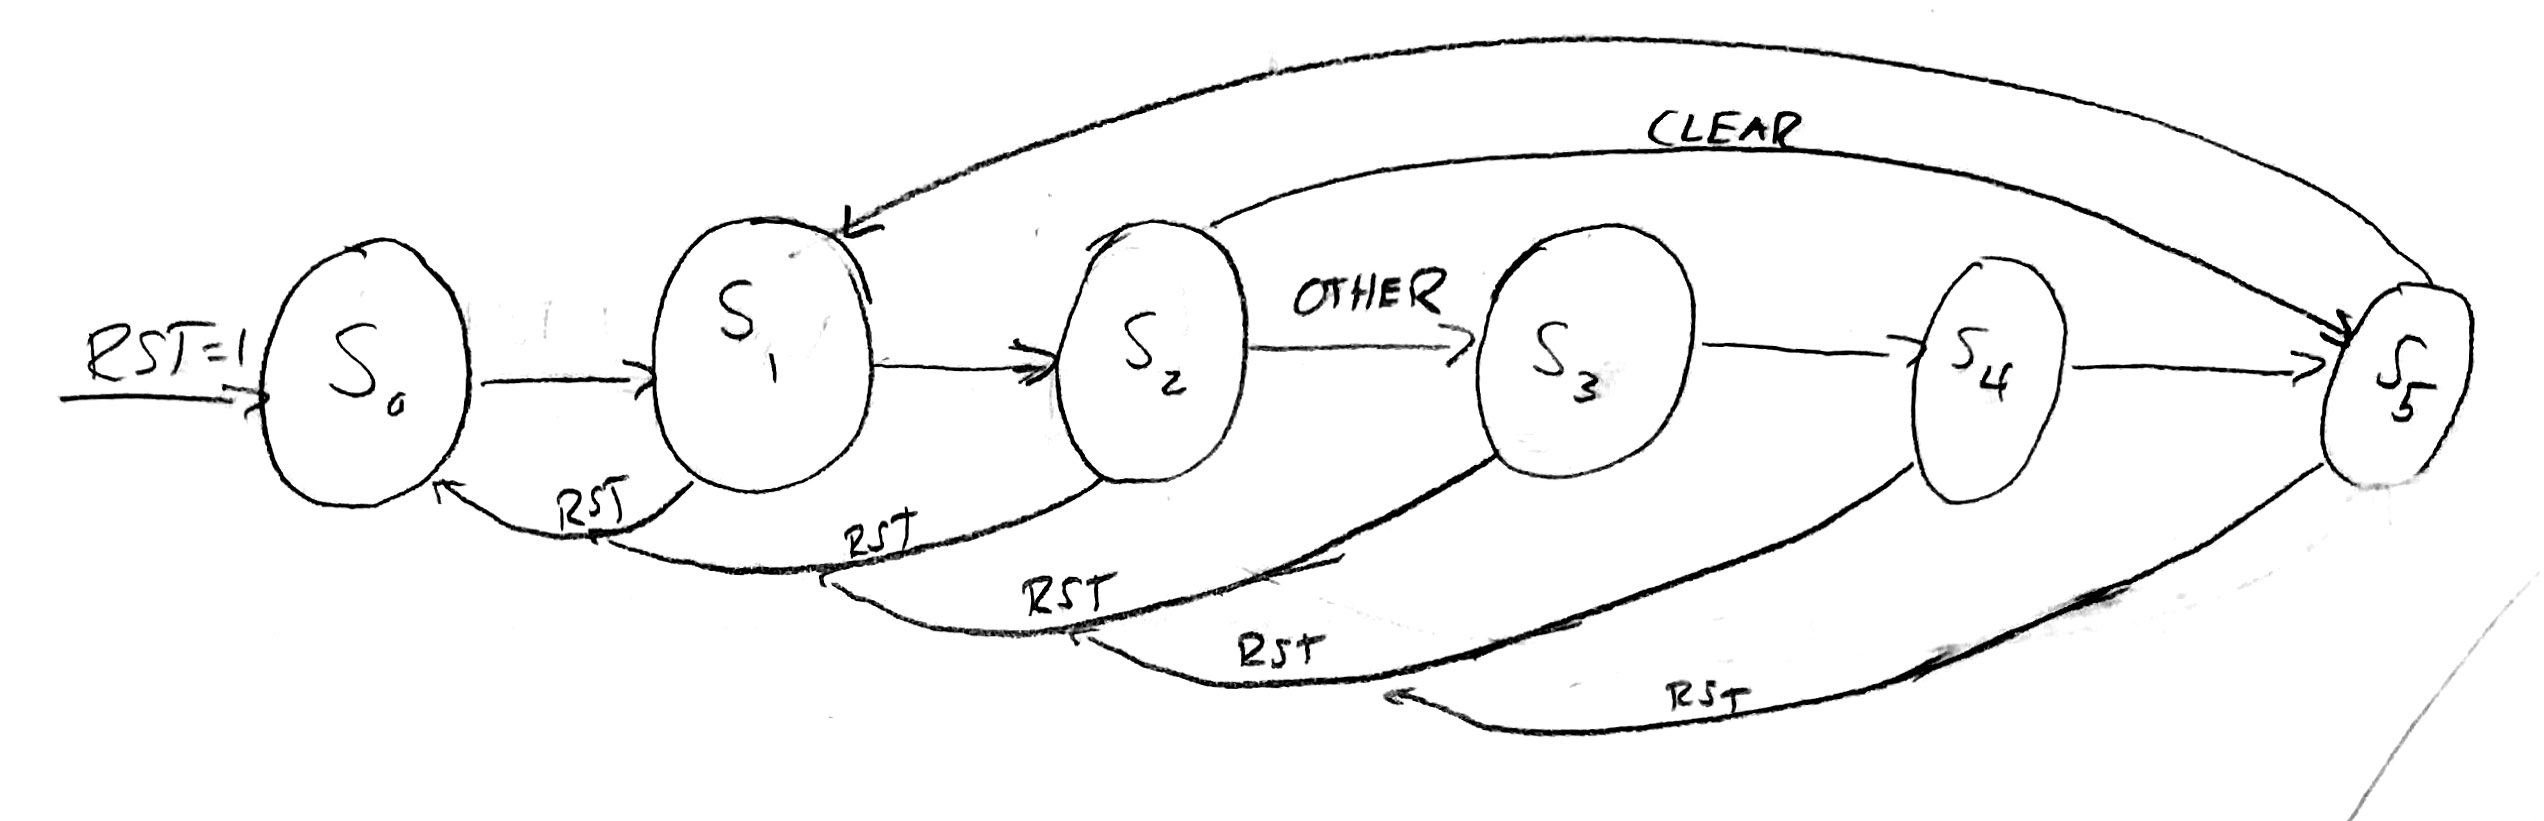
\includegraphics[scale=.18]{Prelab1.jpg}
			\caption{FSM for the controller of the CPU. Created using information from the lecture slides}
		\end{figure}
		\begin{figure}[h]
			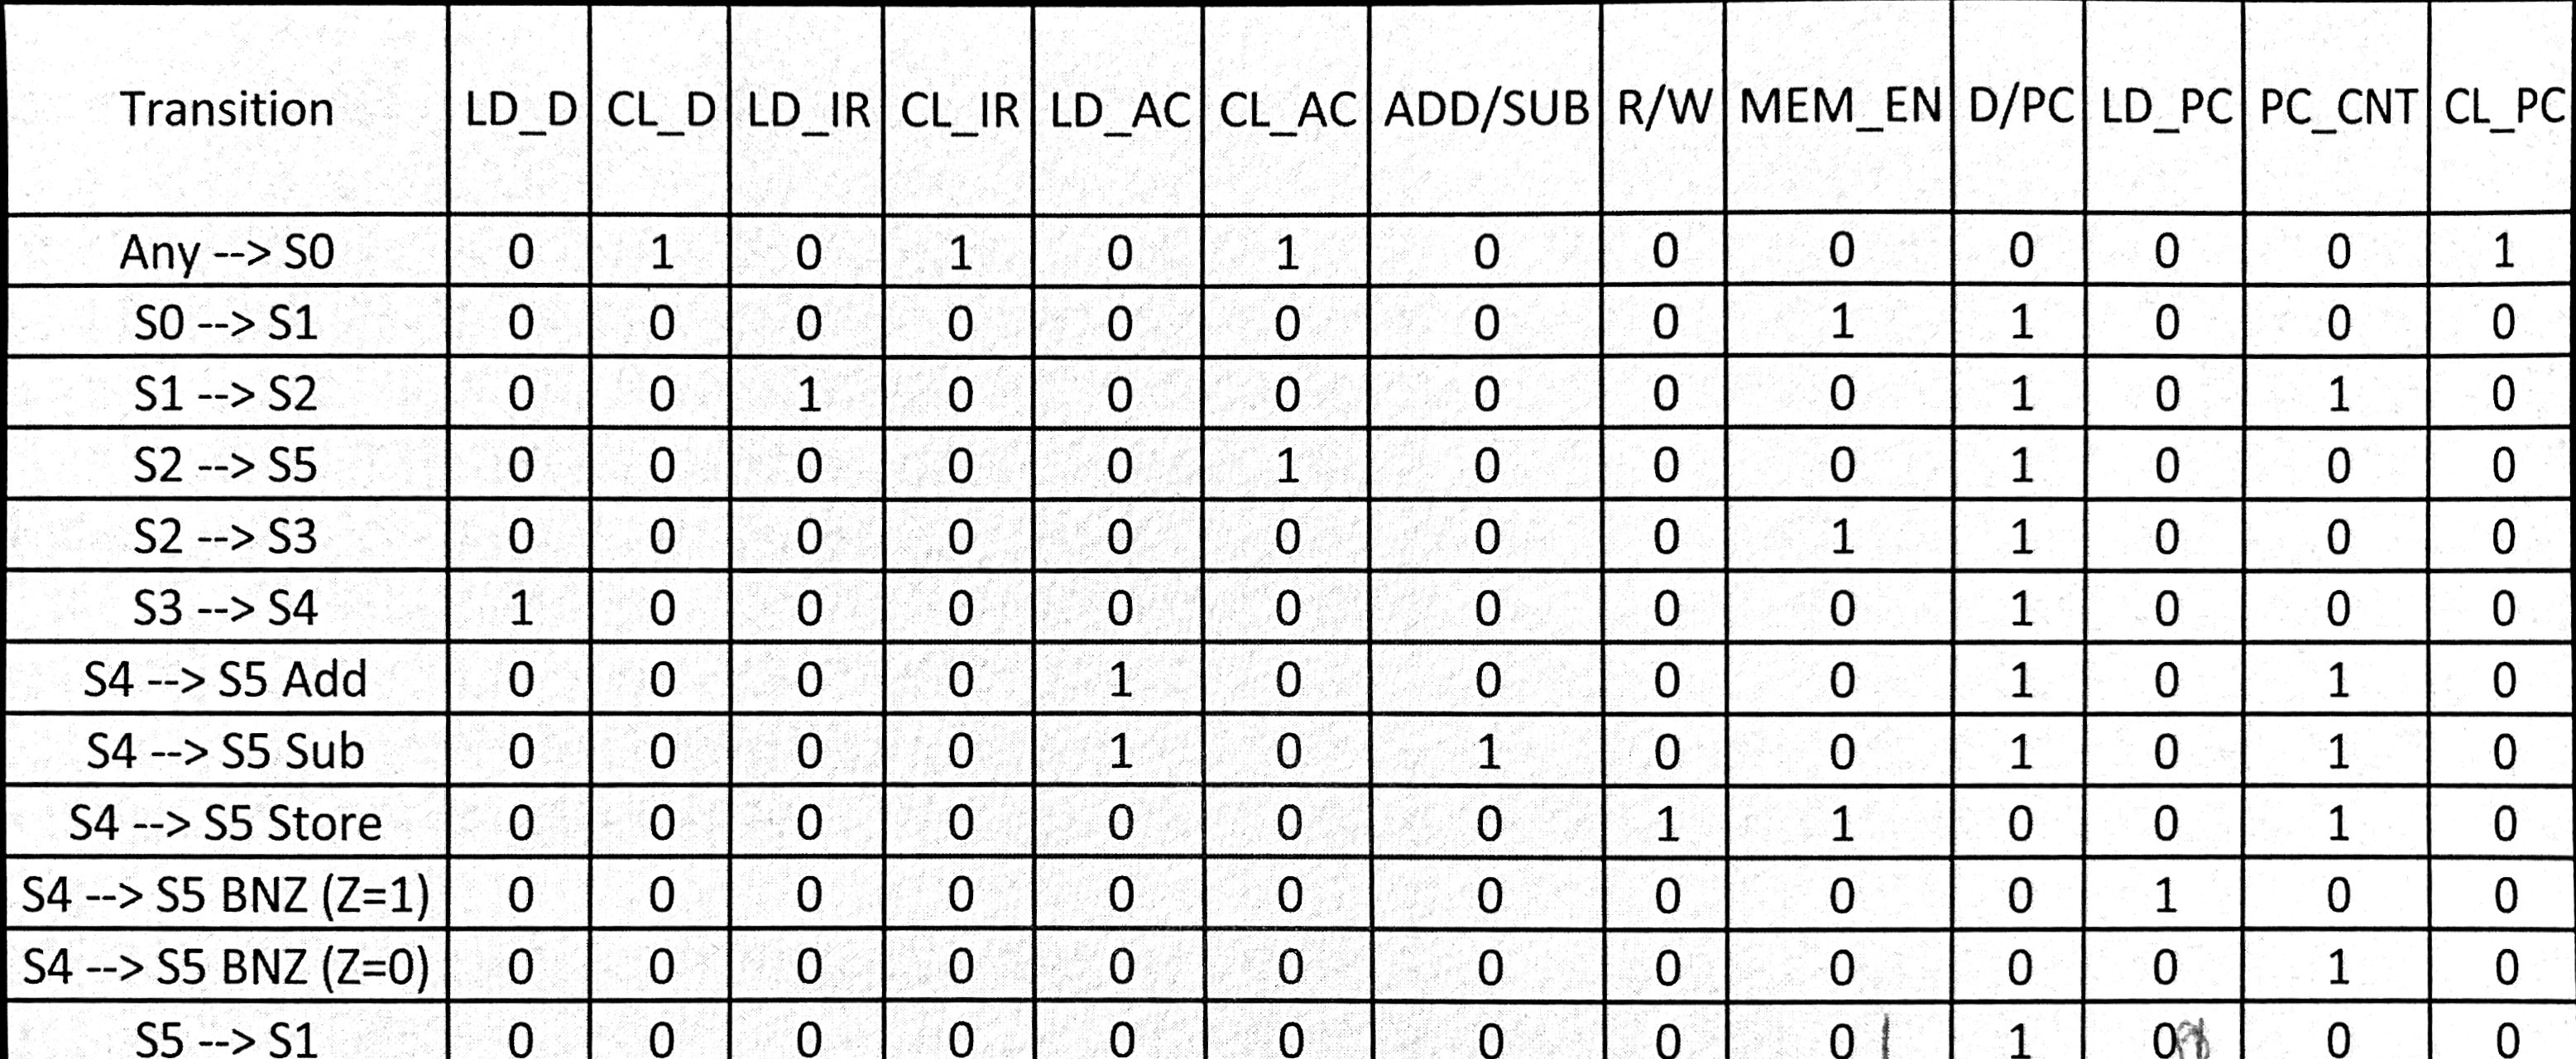
\includegraphics[scale=.15]{Prelab2.jpg}
			\caption{Control Signals. Filled in using states from the lecture slides using one-hot encoding, left any not-on state 0.}
		\end{figure}
		\newpage
		\begin{figure}[h]
			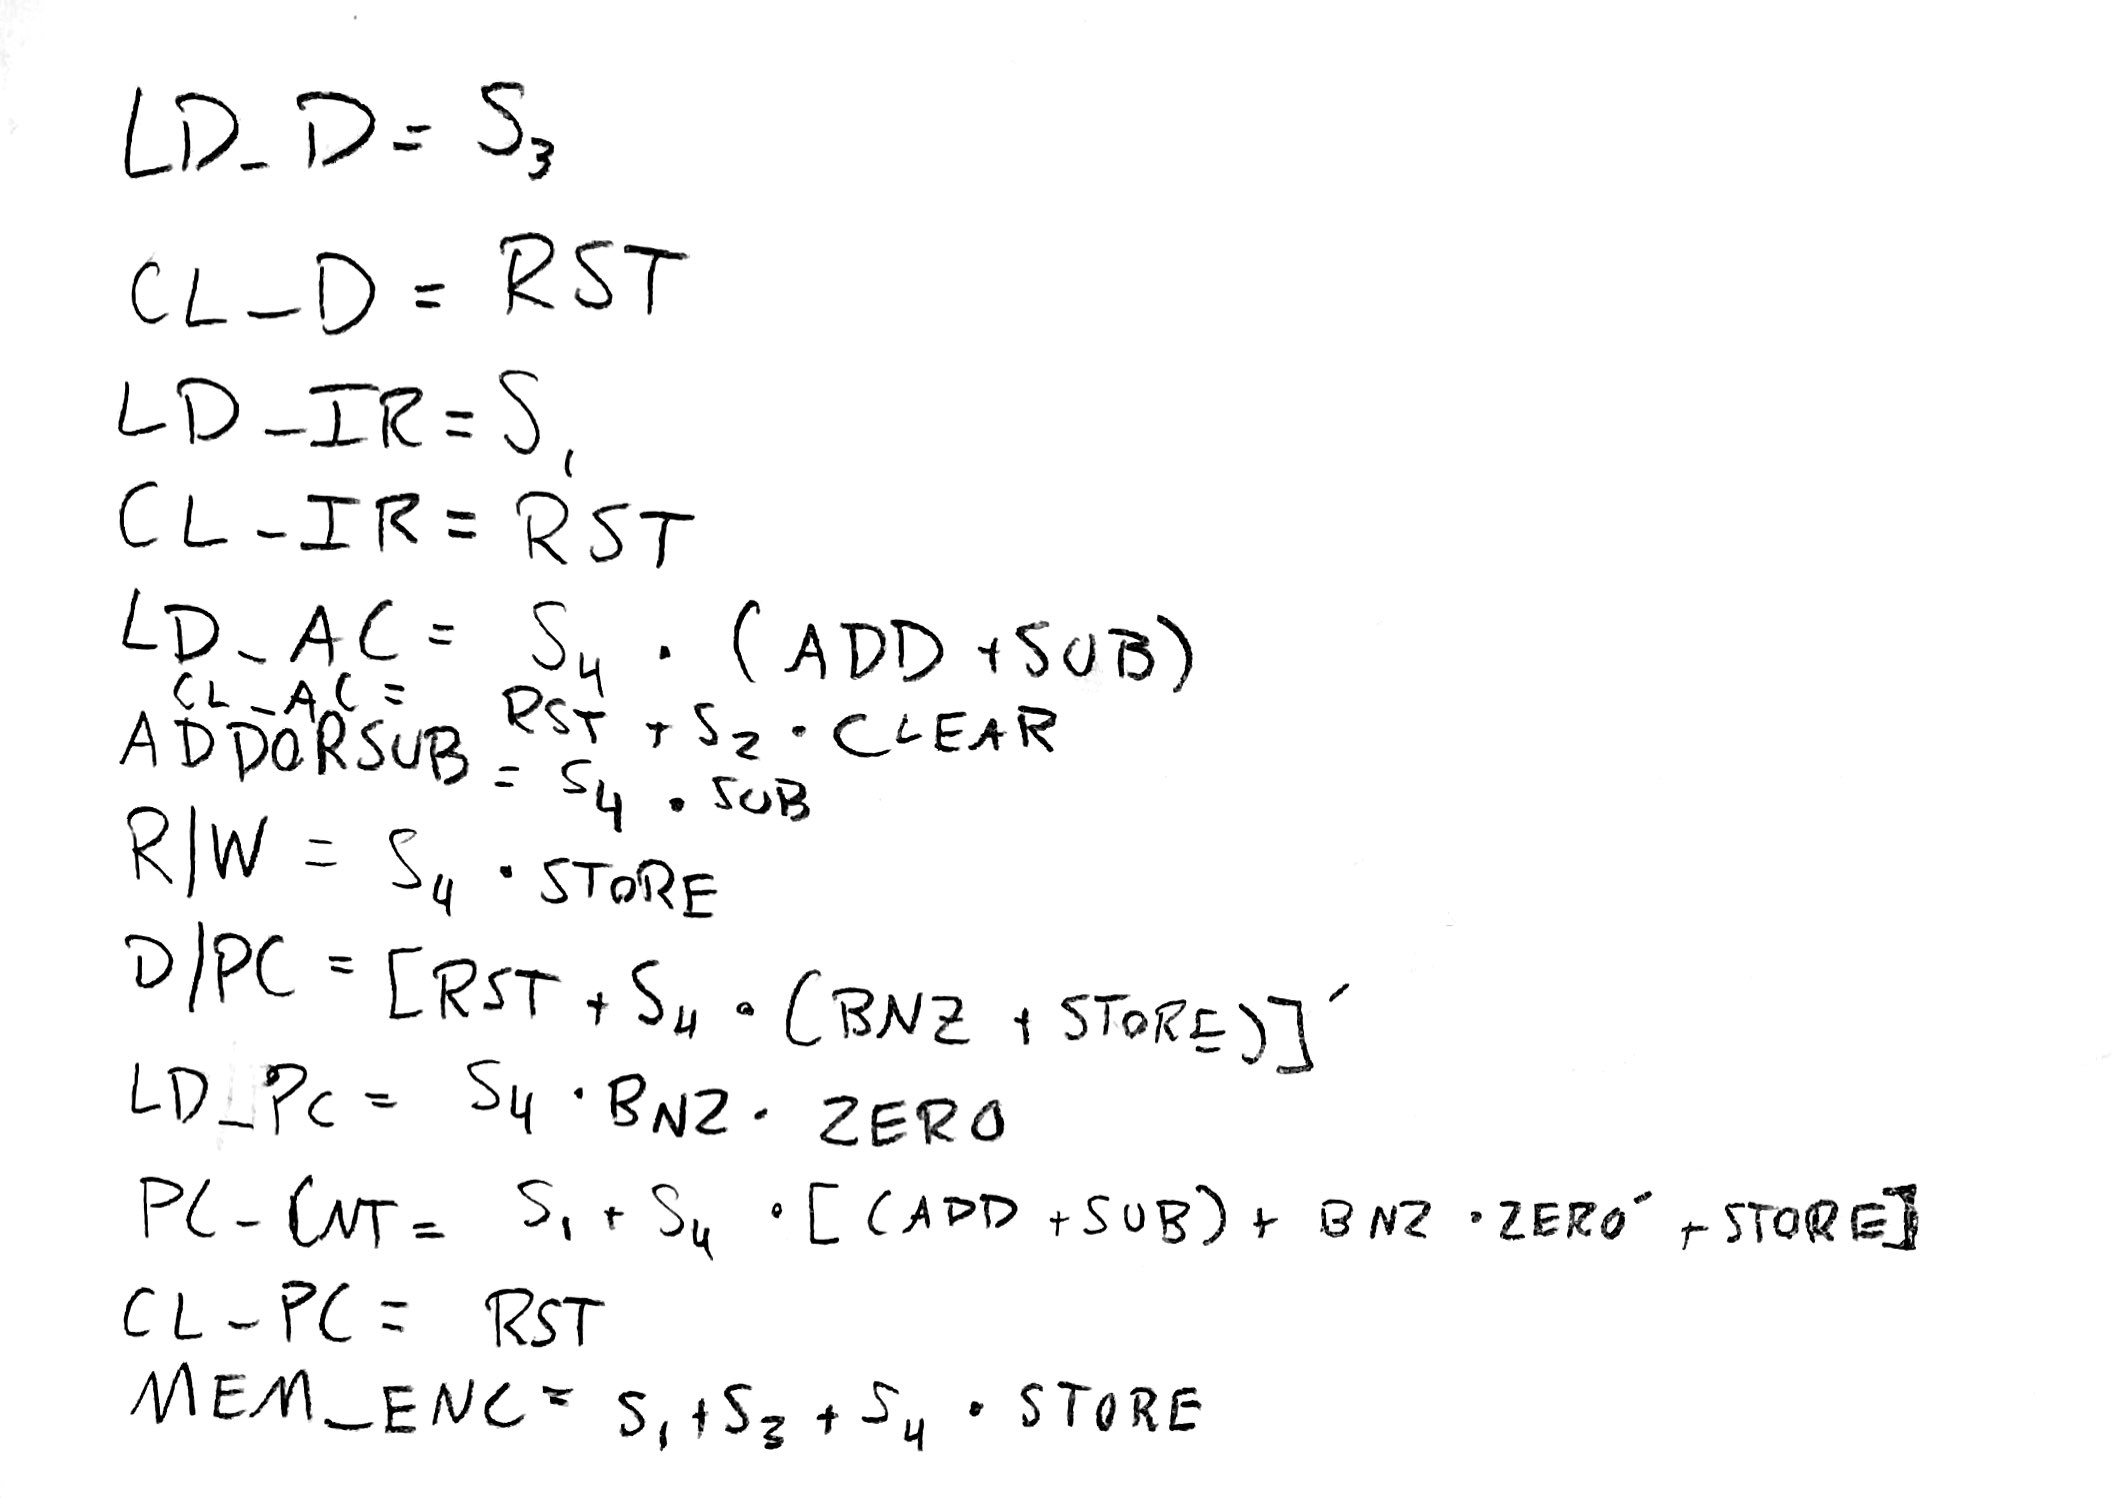
\includegraphics[scale=.13]{Prelab3.jpg}
			\caption{Boolean Equations for figure 2. control signals}
		\end{figure} 

\newpage
		\begin{Verbatim}[frame=single, fontsize= \small]
//control.v
`timescale 1s/1s

module control(CLK,CLR,RESET,S0,S1,S2,S3,S4,S5);
	
	input CLK;
	input CLR,RESET;
	output S0,S1,S2,S3,S4,S5;
	
	reg 	S0,next_S0,
			S1,next_S1,
			S2,next_S2,
			S3,next_S3,
			S4,next_S4,
			S5,next_S5; 
			
	reg 	STATE0,next_STATE0,
			STATE1,next_STATE1,
			STATE2,next_STATE2,
			STATE3, next_STATE3,
			STATE4,next_STATE4,
			STATE5,next_STATE5;

	always @(posedge CLK) 
		begin
			STATE0 = next_STATE0; 
			STATE1 = next_STATE1; 
			STATE2 = next_STATE2; 
			STATE3 = next_STATE3; 
			STATE4 = next_STATE4; 
			STATE5 = next_STATE5; 
			S0 = next_S0;
			S1 = next_S1; 
			S2 = next_S2; 
			S3 = next_S3; 
			S4 = next_S4; 
			S5 = next_S5;
		end
		
	always @ (CLR or RESET or STATE0 or STATE1 or STATE2 or STATE3
	 or STATE4 or STATE5)
		begin
			if ( RESET ) 
				next_STATE0=1;
			else 
				next_STATE0=0;

			if ( ~RESET & STATE0 | ~RESET & STATE5 ) 
				next_STATE1=1; 
			else 
				next_STATE1=0;

			if ( ~RESET & STATE1 ) 
				next_STATE2=1; 
			else 
				next_STATE2=0;

			if ( ~RESET & ~CLR & STATE2 ) 
				next_STATE3=1; 
			else 
				next_STATE3=0;

			if ( ~RESET & STATE3 ) 
				next_STATE4=1; 
			else 
				next_STATE4=0;

			if ( ~RESET & CLR & STATE2 | ~RESET & STATE4 ) 
				next_STATE5=1; 
			else 
				next_STATE5=0;

			if ( RESET ) 
				next_S0=1; 
			else 
				next_S0=0;

			if ( ~RESET & STATE0 | ~RESET & STATE5 ) 
				next_S1=1; 
			else 
				next_S1=0;

			if ( ~RESET & STATE1 ) 
				next_S2=1; 
			else 
				next_S2=0;

			if ( ~RESET & ~CLR & STATE2 ) 
				next_S3=1; 
			else 
				next_S3=0;

			if ( ~RESET & STATE3 ) 
				next_S4=1; 
			else 
				next_S4=0;

			if ( ~RESET & CLR & STATE2 | ~RESET & STATE4 ) 
				next_S5=1;
			else 
				next_S5=0; 
	end
endmodule
		\end{Verbatim}
		Runs through every case assigning states for each possible transition using simple if/else statements. Named each state and transition using variables in verilog. 

	\subsection{Part 2}
		\paragraph*{1-Hot Encoding}
			For this part of the lab we needed to determine how we were going to encode the instruction register and the lab report recommended 1-hot encoding. We have five instructions to encode and an eight bit instruction register so rather than count up by ones we count up in powers of two. This reduces the number of labels sufficently, but we only need five and with counting by powers of two there are eight combinations. This is far easier to construct in a schematic and far more human readible.\\

			\begin{tabular}{c c c}
			\textbf{Instruction} & \textbf{Encoded Value (Decimal)} & \textbf{Encoded Value (Binary)}\\
			\hline
			ADD & 1  & 00000001\\
			SUB & 2  & 00000010\\
			CLR & 4  & 00000100\\
			BNZ & 8  & 00001000\\
			STR & 16 & 00010000\\
			\end{tabular}
		
		\newpage
	\subsection{Part 3}
		
		\begin{figure}[h]
			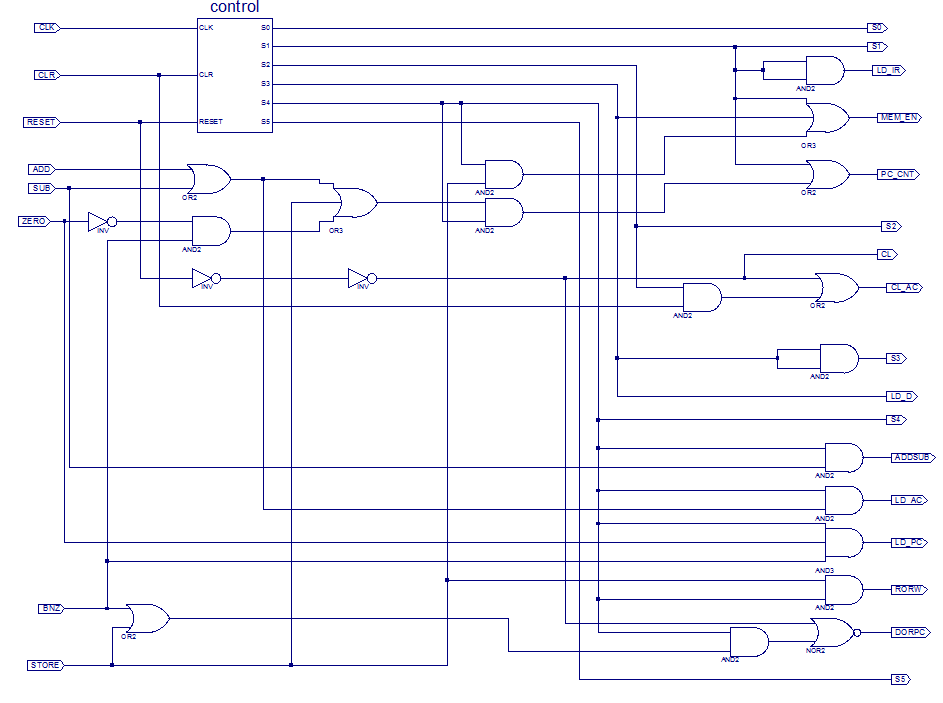
\includegraphics[scale=.6]{controller_sch.png}
			\caption{Shematic for the controller using a symbol for the control module we created in part 1.}
		\end{figure}
		
		\begin{Verbatim}[frame=single, fontsize= \small]
//controller_tb.v
`timescale 1ns/1ps

module controller_tbw_tb_0;

	reg ADD = 1'b0; 
	reg BNZ = 1'b0; 
	reg CLK = 1'b0; 
	reg CLR = 1'b0; 
	reg RESET = 1'b0; 
	reg STORE = 1'b0; 
	reg SUB = 1'b0;	
	reg ZERO = 1'b0; 

	wire ADDSUB; 
	wire CL;
	wire CL_AC; 
	wire DORPC; 
	wire LD_AC; 
	wire LD_D;
	wire LD_IR; 
	wire LD_PC; 
	wire MEM_EN; 
	wire PC_CNT; 
	wire RORW; 
	wire S0;
	wire S1; 
	wire S2; 
	wire S3; 
	wire S4; 
	wire S5;

	initial // Clock process for CLK 
		begin
			forever 
			begin
				CLK = 1'b0;
				#100;
				CLK = 1'b1; 
				#100;
			end
		end
		
	controller_sch UUT( 
		.ADD(ADD), 
		.BNZ(BNZ), 
		.CLK(CLK), 
		.CLR(CLR),
		.RESET(RESET), 
		.STORE(STORE), 
		.SUB(SUB), 
		.ZERO(ZERO), 
		.ADDSUB(ADDSUB), 
		.CL(CL), 
		.CL_AC(CL_AC), 
		.DORPC(DORPC), 
		.LD_AC(LD_AC), 
		.LD_D(LD_D), 
		.LD_IR(LD_IR), 
		.LD_PC(LD_PC), 
		.MEM_EN(MEM_EN), 
		.PC_CNT(PC_CNT), 
		.RORW(RORW), 
		.S0(S0),
		.S1(S1), 
		.S2(S2),
		.S3(S3), 
		.S4(S4), 
		.S5(S5));
	
	initial 
		begin
			// ------------- Current Time: 85ns 
			#85;
			RESET = 1'b1;
			// -------------------------------------
			
			// ------------- Current Time: 285ns 
			#200;
			RESET = 1'b0;
			// -------------------------------------
			
			// ------------- Current Time: 485ns 
			#200;
			CLR = 1'b1;
			// -------------------------------------
			
			// ------------- Current Time: 1085ns 
			#600;
			ADD = 1'b1;
			CLR = 1'b0;
			// -------------------------------------
			
			// ------------- Current Time: 2085ns 
			#1000;
			ADD = 1'b0;
			SUB = 1'b1;
			// -------------------------------------
			
			// ------------- Current Time: 3085ns 
			#1000;
			STORE = 1'b1;
			SUB = 1'b0;
			// -------------------------------------
			
			// ------------- Current Time: 4085ns 
			#1000;
			BNZ = 1'b1;
			STORE = 1'b0;
			// -------------------------------------
			
			// ------------- Current Time: 5085ns 
			#1000;
			ZERO = 1'b1;
			// -------------------------------------
			
			// ------------- Current Time: 5885ns 
			#800;
			ZERO = 1'b0;
			// -------------------------------------
			
			// ------------- Current Time: 6085ns 
			#200;
			BNZ = 1'b0;
			// -------------------------------------
		end 
endmodule
		\end{Verbatim}
		
			
\section{Experimental Results}\vspace{-.7cm} \line(1,0){470}

\begin{figure}[h]
    \centering
	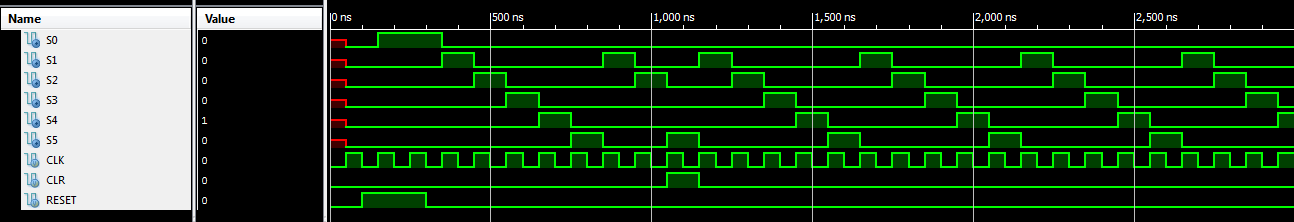
\includegraphics[scale=.48]{control_tb.png}
	\caption{Test bench for the control module. The uniform cascading waves show the simple transitions from 0-5, and at the bottom you can see that when clear is active, S5 occurs, and when reset is active, S0 occurs.}
\end{figure}

\begin{figure}[h]
    \centering
	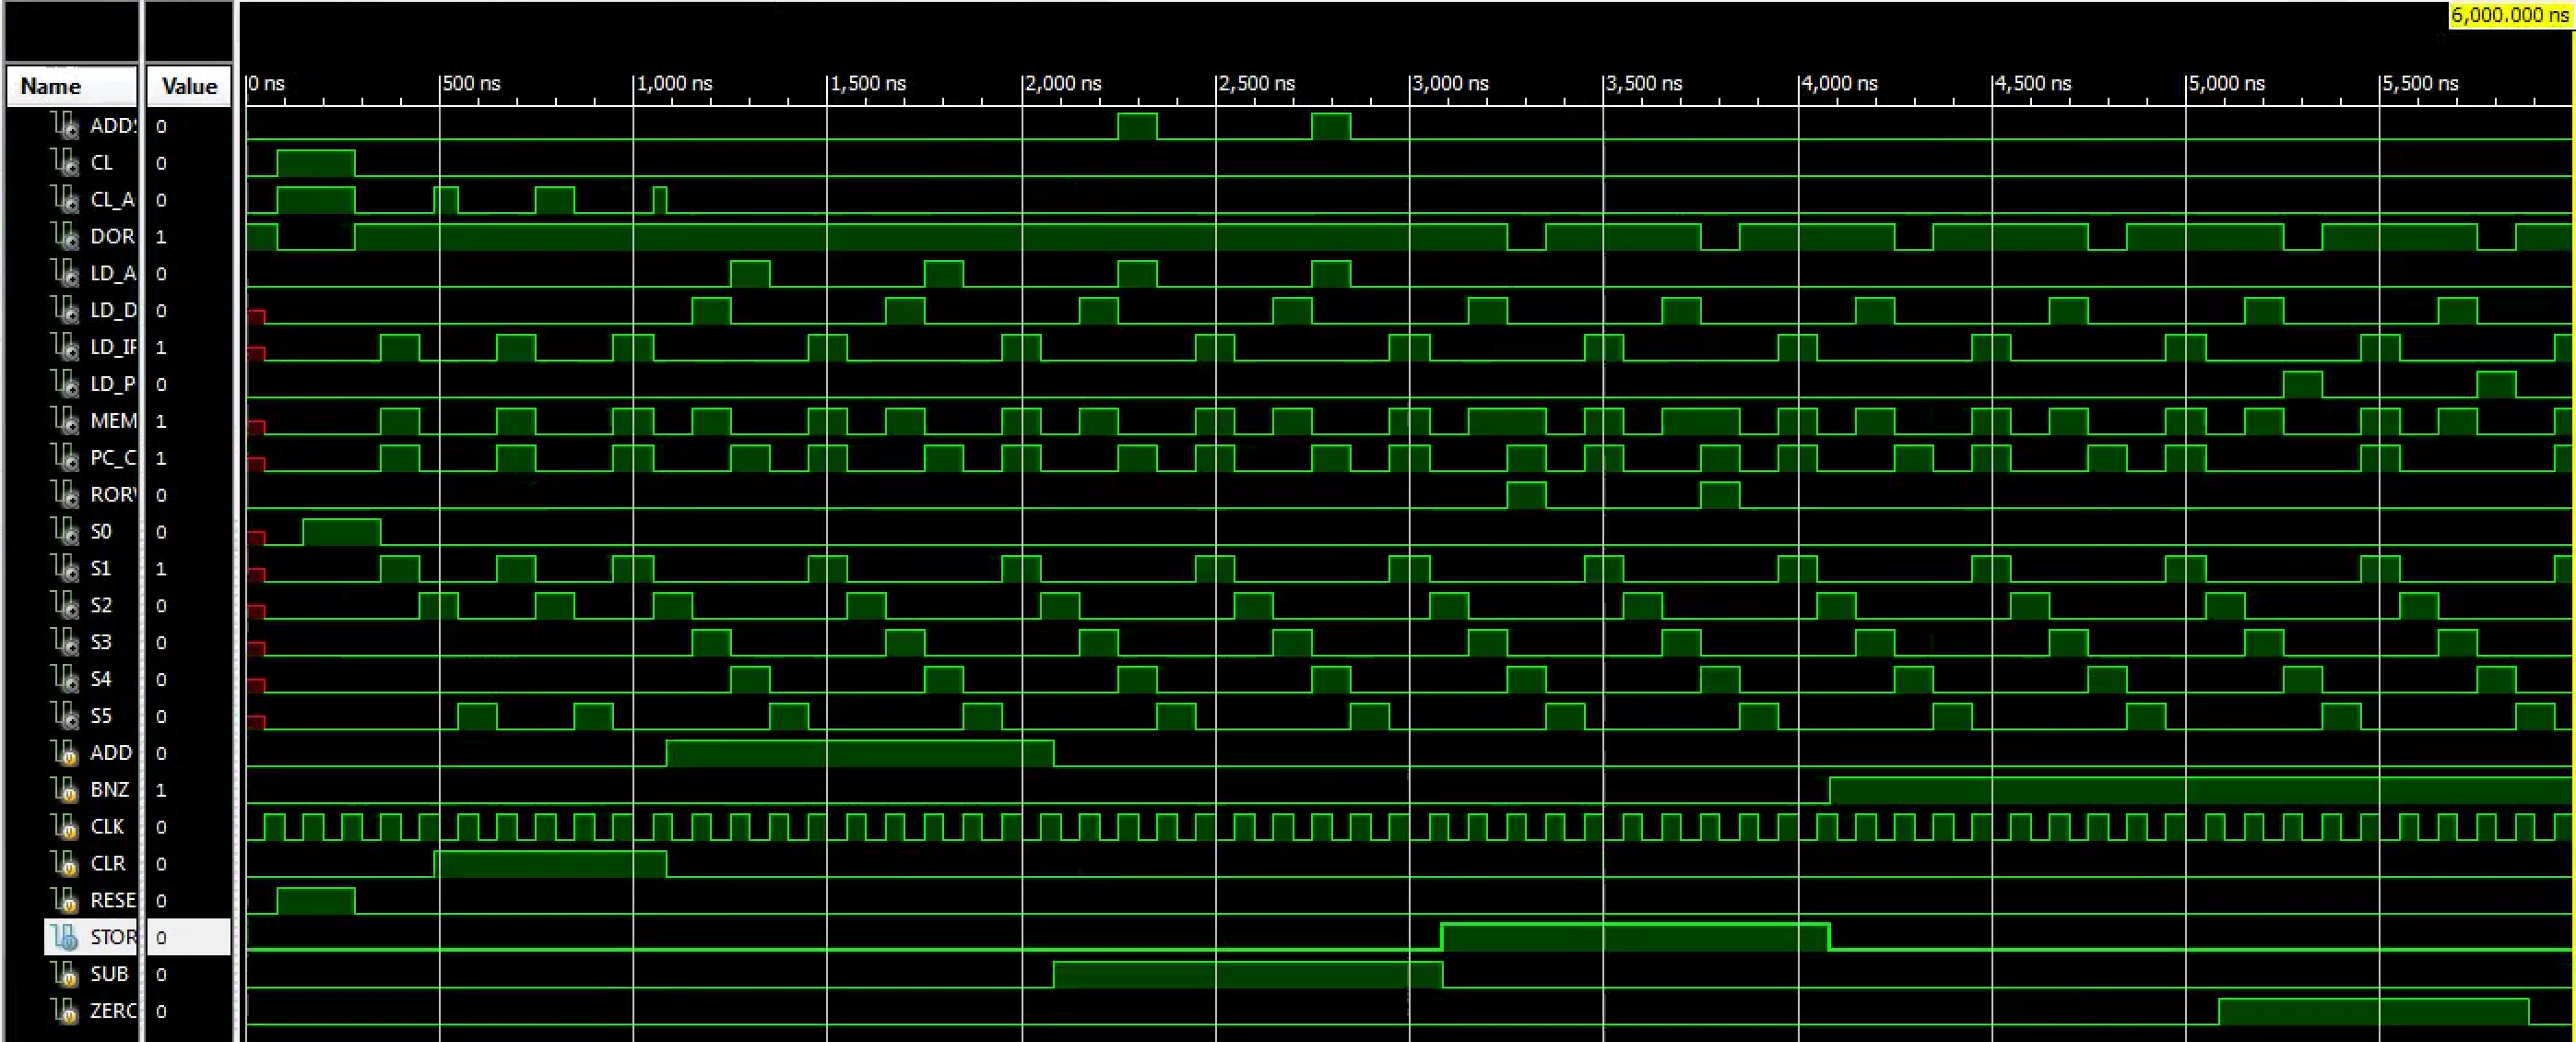
\includegraphics[scale=.33]{controller_tb.png}
	\caption{Test bench for the controller schematic. Cycles clock every 100 ns and changes all states to cover all cases. The inputs line the bottom, and the outputs exist on top. The cascading S0-S5 waves  that look similar to the first test bench are exactly that, more direct state transitions. Then you can see things like CL\_A activating when CLR and S2 are 1, CL on RESET, RORW on STORE and S4, and the rest of the things that occur in the table.}
\end{figure}


	\newpage
\section{Significance} \vspace{-.7cm} \line(1,0){470}
	\paragraph{} Another piece of the full CPU puzzle, the controller allows us to take in any of the control signals and provide the correct instructions to the CPU. With this controller completed, we can move on to connect this portion to the datapath to complete and assemble the toy processor, which will be able to run a given program.


 \section{Comments/Suggestions}\vspace{-.7cm} \line(1,0){470}
 	\paragraph{} 
		
\end{document}


